\Chapter{EXPERIMENTAL RESULTS}\label{sec:SIGNATURE}

Chapter \ref{sec:Approach} introduced four experiments that each address a research questions of this thesis. In adddition to synthetic datasets, they require real datasets.  In this chapter we describe real and synthetic datasets to examine the hypothesis and discuss the results of each experiment.

\section{Data sets}

In experiment 1 we want to extract the predictive performance vector of models over real and synthetic data sets. The performance of the models is assessed over a total of 14~data sets, 7~of which are synthetic, and 7~are real data.  They are listed in table~\ref{tabl1}, along with the number of skills of their Q-matrix, their number of items, the number of the student respondents, and the average score.  Table~\ref{tabl1} also reports the Q-matrix used for each dataset.  As can be seen, some synthetic data sets share their Q-matrix with real data sets.  This sharing allows greater similarity between the synthetic data and a real data counterpart that shares a Q-matrix.  Other parameters used to create the synthetic data sets were also obtained from real data sets with the same intent of allowing better comparison. Chapter \ref{sec:Syn} shows details of generating each synthetic dataset.

Of the 7~real data sets, only three are independent.  The other~4 are variations of a well known data set in fraction algebra from Tatsuoka's work \citep{tatsuoka1984analysis}.  They consists in subsets of questions and variations of the Q-matrix.  These variants allows us to explore the effect of different models (Q-matrices) over the same data source.

The Vomlel data was obtained from \citep{vomlel:2004} and is also on the topic of fraction algebra.  The Q-matrix for this data is derived from the Bayesian Network defined over the 20~item test by experts.

The ECPE data (Examination for the Certificate of Proficiency in English) is an English as a foreign language examination. It is recognized in several countries as a test of advanced proficiency in English and used by a number of universities.

These real data sets were obtained from different sources and are freely available from the CDM \citep{Robitzsch2012} and NPCD ({\url{http://cran.r-project.org/web/packages/NPCD/}}) R packages. The Q-matrices of the real data sets were made by experts.

Note that we use these datasets for experiment 3 which estimates a ground truth model for a dataset based on performance vector classification.

\newcounter{i}\setcounter{i}{1}
\newlength{\mdnum}
\setlength{\mdnum}{\widthof{10}}
\newlength{\mdnumtwo}
\setlength{\mdnumtwo}{\widthof{$\mathbf{Q}_{01}$}}
\newcommand{\mdcount}[2]{\parbox{#1}{\hfill\arabic{i}}.\ #2\addtocounter{i}{1}}
\begin{table}[h]
\centering
\footnotesize
%\begin{tabular}{|l|c|c|r|r|l|}
\begin{tabular}{|l|c|c|r|r|l|}
\hline

%\rowcolor{\color[rgb]{.8,.8,.8}}
\multirow{2}{*}{Data set} & \multicolumn{3}{c|}{Number of} & {\parbox{6ex}{\center Mean\\Score}} & \multirow{2}{*}{Q-matrix}\tabularnewline
\cline{2-4} 
%\rowcolor{\color[rgb]{.8,.8,.8}}
 & Skills & Items & Students &  & \tabularnewline
\hline
\hline
%\rowcolor{\color[rgb]{.9,.9,.9}}
\multicolumn{6}{|c|}{\textit{Synthetic}}\\
\hline
\hline
\mdcount{\mdnum}{Random} & 7 & 30 & 700 &0.75& $\mathbf{Q}_{01}$\tabularnewline
\hline
\mdcount{\mdnum}{POKS} & 7 & 20 & 500 &0.50 & $\mathbf{Q}_{02}$\tabularnewline
\hline
\mdcount{\mdnum}{IRT-2PL} & 5 & 20 & 600 &0.50& $\mathbf{Q}_{03}$\tabularnewline
\hline
\mdcount{\mdnum}{DINA} & 7 & 28 & 500 &0.31& $\mathbf{Q}_5$\tabularnewline
\hline
\mdcount{\mdnum}{DINO} & 7 & 28 & 500 &0.69& $\mathbf{Q}_6$\tabularnewline
\hline
\multicolumn{6}{|l|}{Linear (Matrix factorization)}\\
\hline
\mdcount{\mdnum}{~~~Conj.} & 8 & 20 & 500 &0.24& $\mathbf{Q}_1$\tabularnewline
\hline
\mdcount{\mdnum}{~~~Comp.} & 8 & 20 & 500 &0.57& $\mathbf{Q}_1$ \tabularnewline
\hline
\hline
%\rowcolor{\color[rgb]{.9,.9,.9}}
\multicolumn{6}{|c|}{\textit{Real}}\\
\hline
\hline
\mdcount{\mdnum}{Fraction} & 8 & 20 & 536 &0.53& $\mathbf{Q}_1$\tabularnewline
\hline
\mdcount{\mdnum}{Vomlel} & 6 & 20 & 149 &0.61& $\mathbf{Q}_4$\tabularnewline
\hline
\mdcount{\mdnum}{ECPE} & 3 & 28 & 2922 &0.71& $\mathbf{Q}_3$\tabularnewline
\hline
\multicolumn{6}{|l|}{Fraction subsets and variants of $\mathbf{Q}_{1}$}\\
\hline
\mdcount{\mdnum}{~~~1} & 5 & 15 & 536 &0.53& $\mathbf{Q}_{10}$\tabularnewline
\hline
\mdcount{\mdnum}{~~~2/1} & 3 & 11 & 536 &0.51& $\mathbf{Q}_{11}$\tabularnewline
\hline
\mdcount{\mdnum}{~~~2/2} & 5 & 11 & 536 &0.51& $\mathbf{Q}_{12}$\tabularnewline
\hline
\mdcount{\mdnum}{~~~2/3} & 3 & 11 & 536 &0.51& $\mathbf{Q}_{13}$\tabularnewline
\hline
\hline
\end{tabular}
\caption{Datasets}
\label{tabl1}
\end{table}

The synthetic data sets are generated from each skills assessment model, with an effort to fit the parameters as closely as possible to a real data counterpart that shares the same Q-matrix.  

For POKS, the structure was obtained from the Fraction data set and the conditional probabilities were generated stochastically, but in accordance with the semantic constraints of these structures and to obtain an average success rate of 0.5.

For IRT, the student ability distributions was obtained from the Fraction data set, and the item difficulty was set to reasonable values: averaging to 1 and following a Poisson distribution that kept most values between 0.5 and 2 (done by generating random numbers from a Poisson distribution with lambda parameter set to 10 and dividing by 10). 

The synthetic datasets from linear and Cognitive Diagnosis models were generated by taking a Q-matrix of 7~skills that contains all possible combinations of 1 and 2~skills, which gives a total of 28~combinations and therefore the same number of items. For skills mastery we set $\alpha_I$, $\beta_I$, $\alpha_S$ and $\beta_S$ parameters equal to $1.5$ to avoid high or low entropy for student and item variance. Skills space for DINA/DINO models considers all possible combination of skills with same probability of appearance in the skills mastery matrix. 
The synthetic datasets with linear model ground truths do not have any noise factor where \textit{slip} and \textit{guess} values of $0.1$ and $0.2$ respectively were set for synthetic data with DINA and DINO models.

Note that the first 3~models (Expected, IRT, POKS) do not rely on any Q-matrix neither for the data generation process nor for learning phase, but the DINO/DINA and matrix factorization assessment models still require one during the learning phase. For example a synthetic data with IRT model does not accompany any Q-matrix to preform experiment 1 which is assessing predictive performance vector of models but DINA requires one in the learning phase of this experiment. To define these Q-matrices (denoted~$\mathbf{Q}_{0x}$ in table~\ref{tabl1}, a wrapper method was used to first determine the number of skills according to \citet{Beheshti2012Numbers}, then a Q-matrix was derived with the deterministic ALS algorithm (see \citealp{Desmarais2013aied}, for more details on ALS technique), starting with an initial random Q-matrix.



%%%%%%%%%%%%%%%%%%%%%%%%%%%%%%%%%%%%%%%%%%%%%%%%%%%%%%%%%%%%%%%%%%%%%%%%%%%%%
\section{Results of Experiment 1: Predictive performance of models over real and synthetic datasets} \label{secSyn}

There are two possibilities for visualization of the predictive performance of seven models over a dataset, Figure \ref{Fig:Predictive-Preformace_rep} shows these two representations of the same results data. We used both of them in this thesis, whichever is deemed more appropriate to ease understanding. Figure \ref{Predictive-Preformace_Sig} shows the signature performance in terms of percent accuracy of seven models over a dataset. Figure \ref{Predictive-Preformace_Base} centers the performances with respect to the accuracy of the \textit{expected} model which serves as a baseline.  When a model performs below that performance, it can be considered a relatively weak performer since the expected value is simply the combined student and item mean.

\begin{figure}[h]
\centering
 \subfigure[Absolute accuracy percentage.]{
   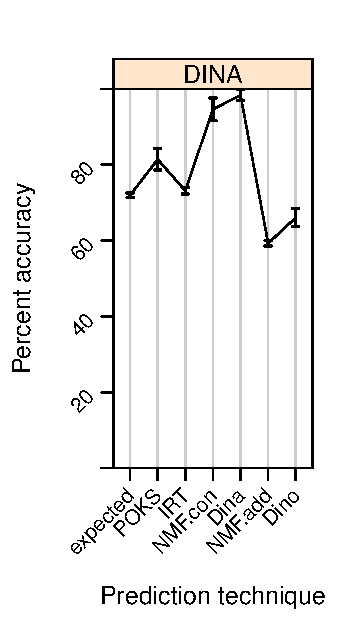
\includegraphics[scale =1] {Predictive-Preformace_Sig.pdf}\label{Predictive-Preformace_Sig}
 }\quad
\subfigure[Relative accuracy (centered at the \textit{expected} model performance).]{
   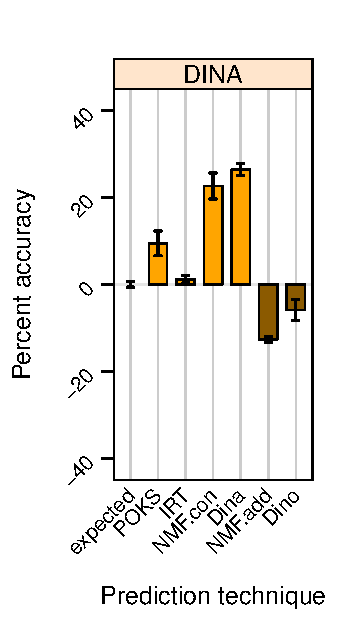
\includegraphics[scale =1] {Predictive-Preformace_Base.pdf}\label{Predictive-Preformace_Base}
 }
\caption{Two types of representation of predictive performance of 7 models over DINA generated dataset}
\label{Fig:Predictive-Preformace_rep}
\end{figure}


\begin{figure}
\centering
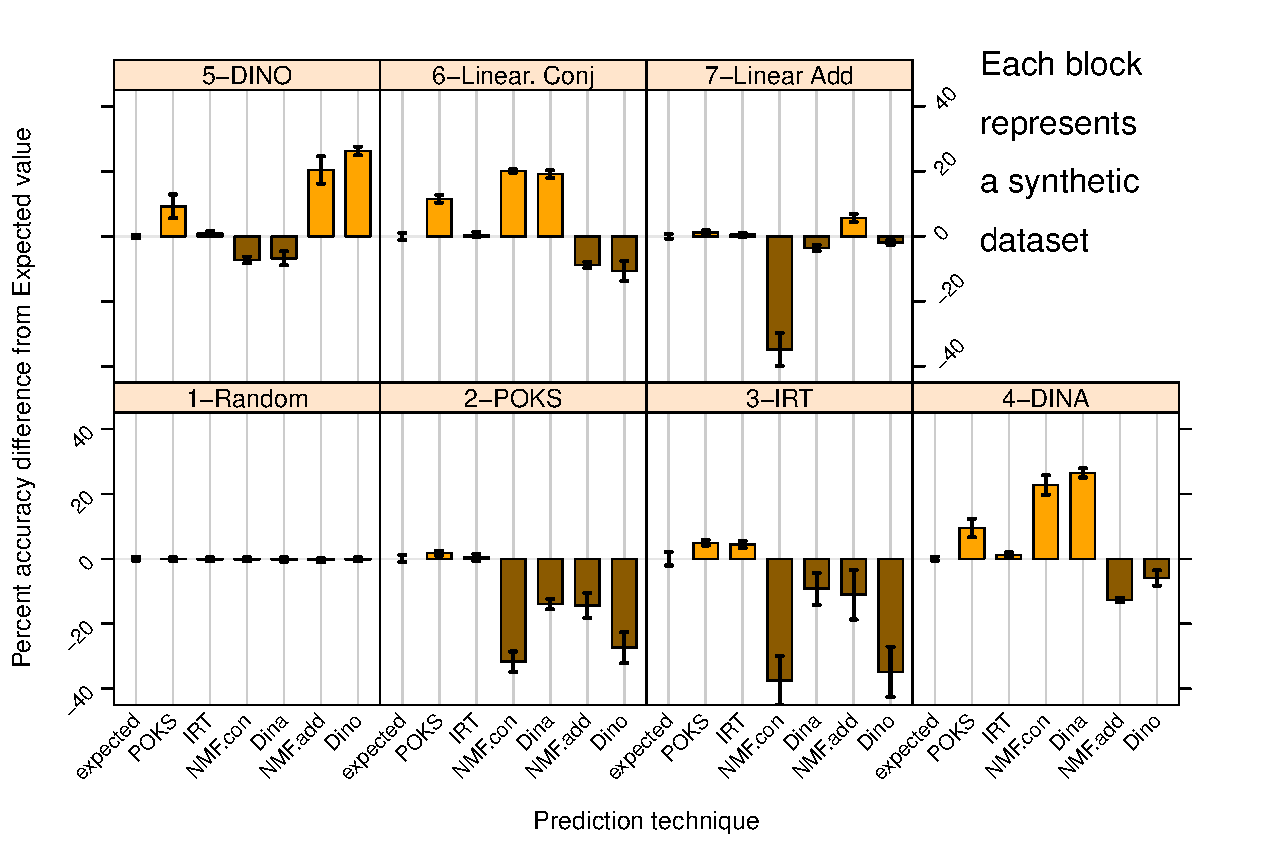
\includegraphics[clip=true,width=.9\textwidth]{Syn.pdf}
\caption{Item outcome prediction accuracy results of {\textbf{synthetic data sets}}}
\label{fig1}

{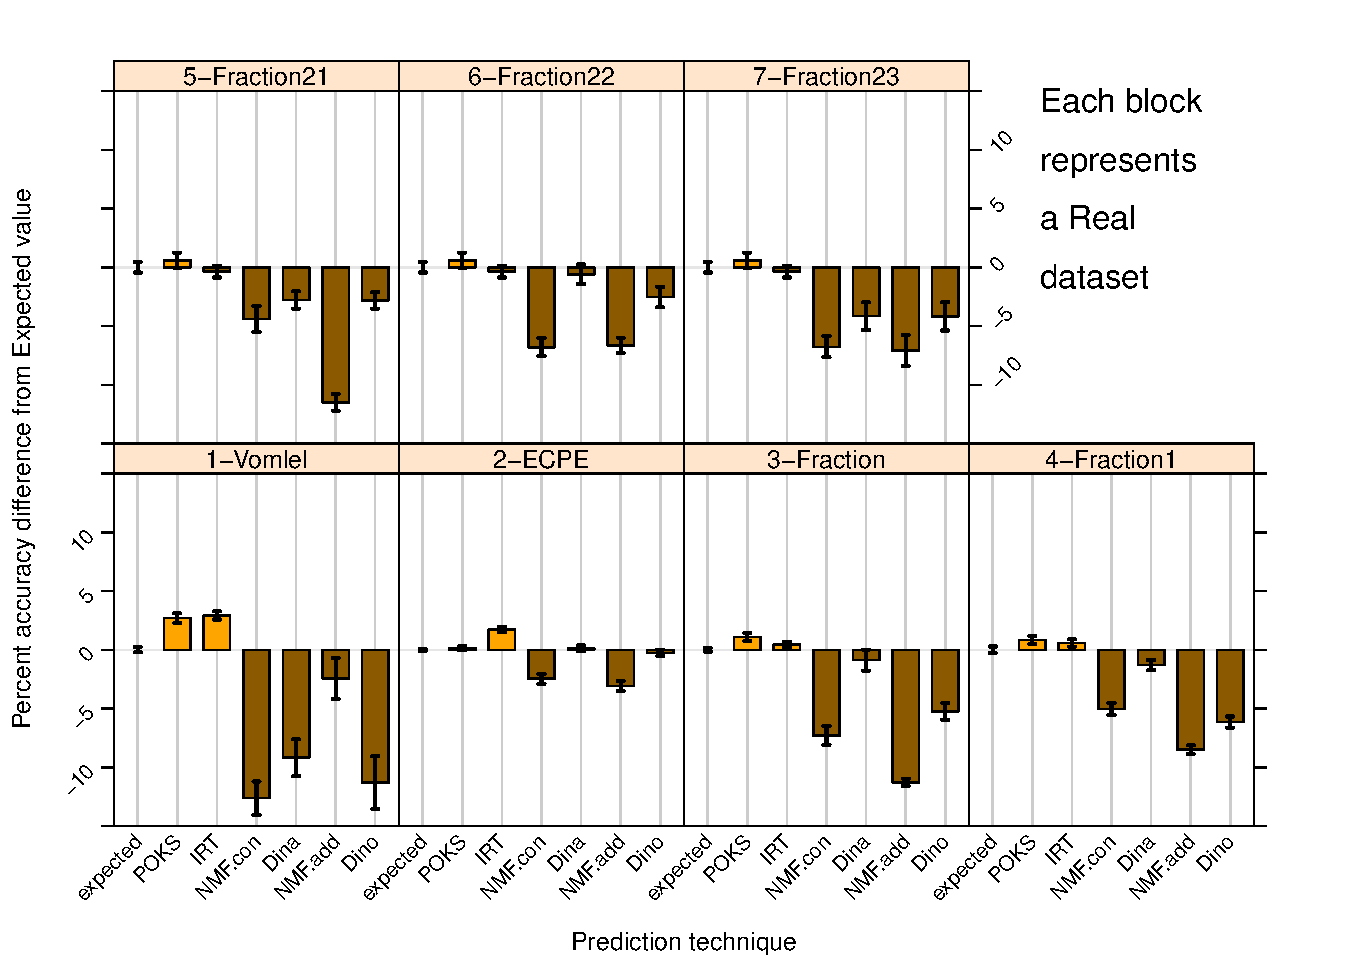
\includegraphics[clip=true,width=.9\textwidth]{Real.pdf}}
\caption{Item outcome prediction accuracy results of {\textbf{real data sets}}.  Note that the y-scale is different than the synthetic data set.}
\label{fig2}
\end{figure}


Figures~\ref{fig1} and~\ref{fig2} show the performance of each model over the synthetic and real data sets described in table~\ref{tabl1}. Note that the y-scale of the synthetic data is double the one of the real data sets, and therefore the differences in performance for the synthetic datasets are much wider.  An error bar of 1~standard deviation is reported, computed over 10 simulation runs that each run considers four different number of observation that varies between 9 to an item less than the maximum number of items, provides an idea of the variability of the results. A dataset of random data is also reported for a~$0.75$ average success rate.

\note{If you have the scripts to quickly produce the figures, it would be worth using a 95\% confidence interval which is the standard deviation divided by the square root of the number of instances (10).  A 95\% c.i. is 2 standard deviations and the sqrt of 10 is about 1/3, so the bars should be around 2/3 of the ones shown.  If recreating these figures is too much work, we can simply mention this fact.}


\subsection{Discussion}

For the synthetic data sets, as expected, when the generative model behind the data set is the same as the skills assessment technique, the corresponding technique's performance is the best, or close to the best.  And this performance is also always above the expected value performance, except for the random data set where no model can do any different than the expected value, which is what we would expect.

Three models reach performances that are much higher than the baseline, in the range of $20-30$\% (DINO, Linear Conjunctive, and DINA), whereas for the three other models the gain is closer to 5\% (Linear additive, POKS, and IRT).

An important observation is that the pattern of relative differences of performances across techniques varies considerably and is unique to each data set: no two data sets have the same pattern of performance vector across models.  The capacity of recognizing a data set's true model relies on this uniqueness characteristic.

For the real data sets, the performance vector among the techniques shows smaller discrepancies and is closer to the baseline. 

An interesting finding is that in most cases, the best performer is close to the baseline. Moreover, a majority of models do worst than the baseline on most of data sets. This is particularly surprising for the DINA model which is a relatively well accepted model in psychometrics and student modeling.  Even the highly used IRT model is not showing a better performance than the \textit{expected} model.  This is due in part because the estimated from \textit{expected} model can rely on at least 19~observed items, but it is still indicative of a weakness of the models when we compare these results with the synthetic data results where the underlying model often reaches 20\% above the \textit{expected} baseline.  Also noteworthy to notice is that for the POKS and IRT synthetic data, the highest performances are notably lower than for the other models.  We will study in a later experiment the performances when fewer items are observed.

\note{It is surprising that POKS does not do any better, and even worst than Vomlel.}

\note{Where is the mention that the target item to predict is the last one?  Or is it?  It would be worthwhile to provide more details on this in this chapter or the previous.}

The results from the subsets of the Fraction data show that the pattern of the Fraction performance data set repeats over Fraction-1, Fraction-2/1 and Fraction-2/2, in spite of the different number of skills and different subsets of questions.  However, it differs substantially from Fraction-2/3 for the NMF conjunctive performance which reaches that of the NMF additive one and also DINA reaches DINO. This is readily explained by the fact that the Q-matrix of this data set has the property of assigning a single skill to each item, in which case the two matrix factorization techniques or even cognitive diagnosis models become equivalent.  But aside from the Fraction-2/3 case, this similarity among Fraction data set and its derivative suggests that in spite of the model differences (different Q-matrices and item subsets), the performance ``signature'' remains constant across these data sets.

Finally, we note that none of the real data sets show the large the amplitude and the differences found in the synthetic data sets models (the scale of figure~\ref{fig1} is about 4 times that of figure~\ref{fig2}). One exception is the IRT synthetic data set which displays smaller variance across models and which ``signature'' resembles the Vomlel data, although the performance difference with the majority class is substantially higher for the synthetic data than the Vomlel data, suggesting that the real data is yet not a perfect fit to this model. Details of this conclusion is given in the next section.\note{I do not get to the same observations here.}


\section{Results of Experiment 2: Sensitivity of the Model performance over data generation parameters}
\label{Sensitive}

The results of previous experiment show that the performance signature pattern is unique to each dataset among datasets with different ground truths. The next question to address is whether they are stable in addition to be unique.  This question motivated us to test the sensitivity of this pattern over wide span of data generation parameters. Therefore in this experiment we generated synthetic datasets with different conditions of the parameters that is presented in table~\ref{fig:param}. We should note that all other parameters are set to a default value while we are testing a specific parameter.

\begin{table}[h]
  \centering

  \begin{tabular}{>{\raggedright}p{.02\textwidth}>{\raggedright}p{.3\textwidth}>{\raggedright}p{.15\textwidth}>{\raggedright}p{.4\textwidth}}
    \toprule
    & \multicolumn{1}{c}{\textbf{Parameter}} & \multicolumn{1}{c}{\textbf{Typical values}} & \multicolumn{1}{c}{\textbf{Models affected}} \tabularnewline
    \toprule
    \multicolumn{3}{l}{\textbf{Data specific parameters}}\tabularnewline
    \cline{2-4}
    & Number of skills & \numrange{3}{9} & Multiple skills models:\newline DINA, DINO, NMF Conj./Add. \tabularnewline
    \cline{2-4}
    & Number of items & \numrange{10}{50} &   \tabularnewline
    \cline{2-3}
    & Number of students & \numrange{100}{1500} & \tabularnewline
    \cline{2-3}
    & Test success rate & \numrange{0.25}{0.85}   &\tabularnewline
    \cline{2-3}
    & Student score variance & \numrange{0.03}{0.20} & \tabularnewline
    \cline{2-3}
    & Item score variance & \numrange{0.03}{0.20} & \multirow{-5}{*}{All models} \tabularnewline
    \cline{2-4}
    & Item discrimination & \numrange{0.5}{3} & \tabularnewline
    \cline{2-3}
    & Item difficulty & \numrange{-3}{3} & \tabularnewline
    \cline{2-3}
    & Student ability & \numrange{-4}{4} & \multirow{-3}{*}{IRT} \tabularnewline
    \hline
    \multicolumn{3}{l}{\textbf{Simulation parameters}}\tabularnewline
    \cline{2-4}
    & Number of observed items &  9 to Number of items -1 & \tabularnewline
    \cline{2-3}
    & Training set size & 90\% of $[100-1500]$ &  \multirow{-2}{*}{All models}\tabularnewline
    \hline
    \multicolumn{3}{l}{\textbf{Model specific parameters}}\tabularnewline
    \cline{2-4}
    & Guess and slip & $[0.0-0.2]$ & DINO and DINA\tabularnewline
    \cline{2-4}
    & Binomial and interaction tests & $\alpha_1=0.85\newline \alpha_2=0.10$ & POKS\tabularnewline
    \bottomrule
  \end{tabular}
  \caption{Parameters of the simulation framework}
  \label{fig:param}
\end{table}


Akin to the previous experiment we assessed the predictive performance signature of these datasets on the basis of 10-folds cross-validation. We also fixed the number of ``observed items'' for each run on each data set that varies between 9 to one item less than total number of items.



\subsection{Results and discussion}

\note{Why not name ``Bayesian generated'' simply ``POKS''?  It is hart for the reader to make the link.}

Figure~\ref{figSampleSize} shows the results of extracting performance signature from datasets with different number of students. Obviously, the signature pattern did not change significantly except for IRT-based generated dataset for small sample size\note{I do not see this??}. 

\begin{figure}
  \centering

    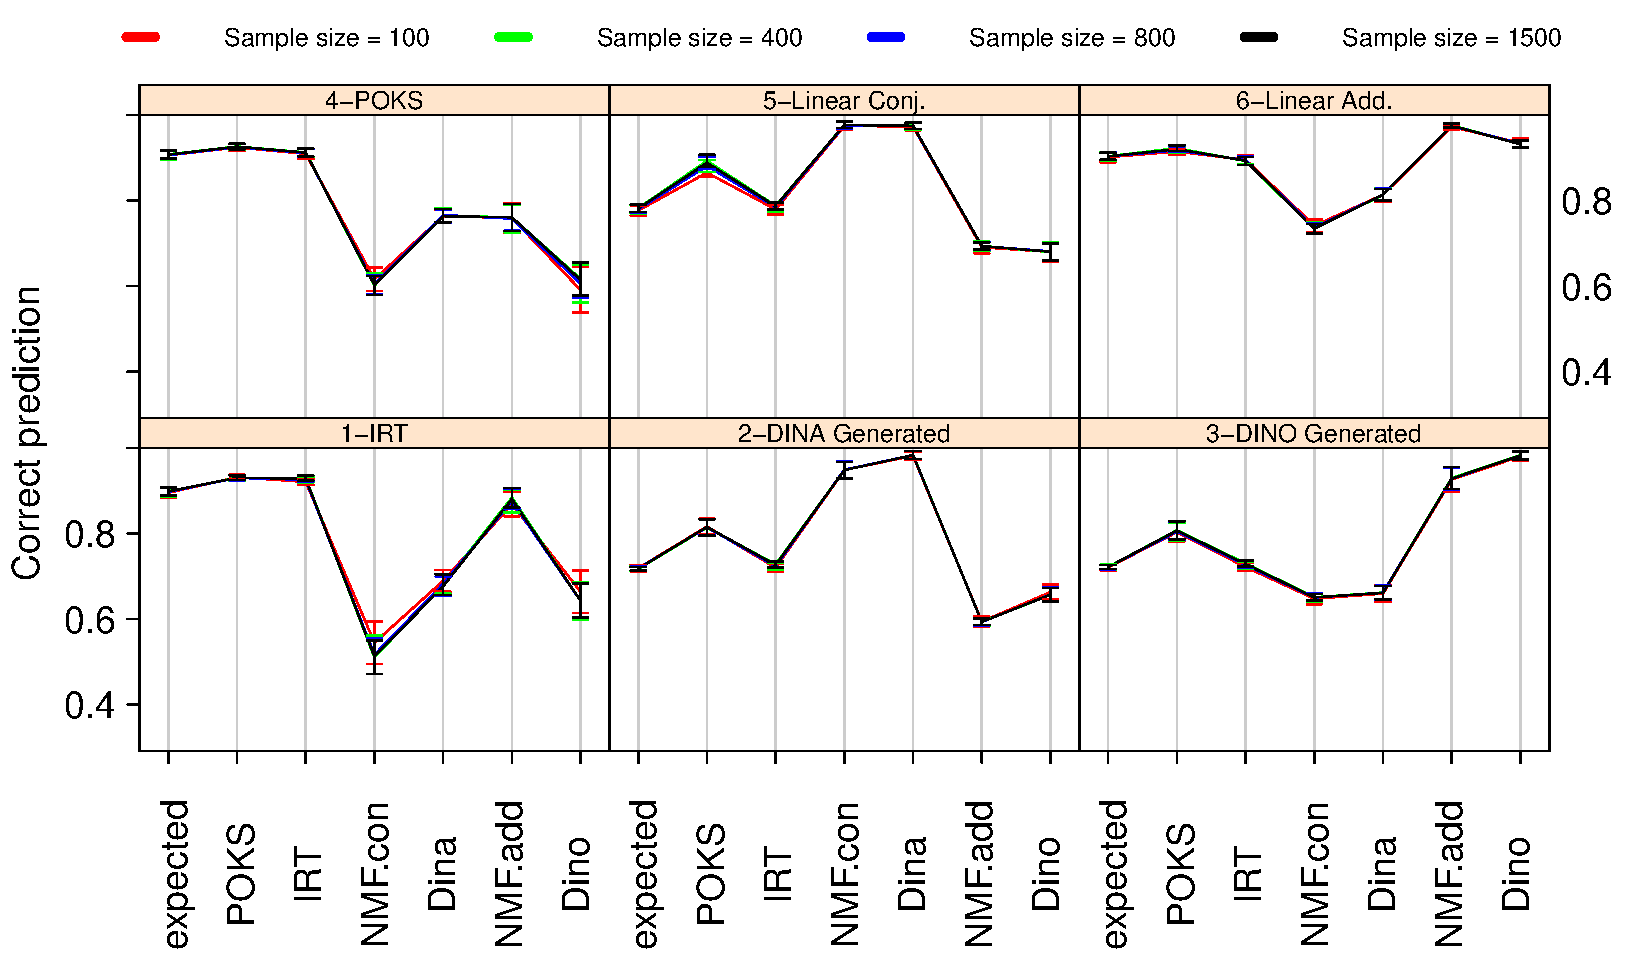
\includegraphics[scale=0.58]{SampleSize.pdf}
     \caption{Variation of \textbf{Sample Size} Over synthetic data sets}
\label{figSampleSize}
\end{figure}


\note{Next paragraph: This is the number of items observed, right? Not the number of items in total.  And what are/is the target item/s?  Is it still a single item, such as the last unobserved one?  And if it is a single one, is it always the same one? chosen at random?}

The other parameter is the number of items. Figure~\ref{figNumberofItems} shows how the performance signature has been changed on different parameter assumptions. For three types of synthetic data (IRT, POKS, Linear additive) the pattern of the signature does not change across this parameter but for the others ( Linear Conj. DINA, DINO) it shifts down once the number of items degrades. This result highlights the role of this parameter in the assessment of performance vector. It also shows that even for synthetic data the ground truth should not necessarily be close to 100\%.

\begin{figure}
  \centering
    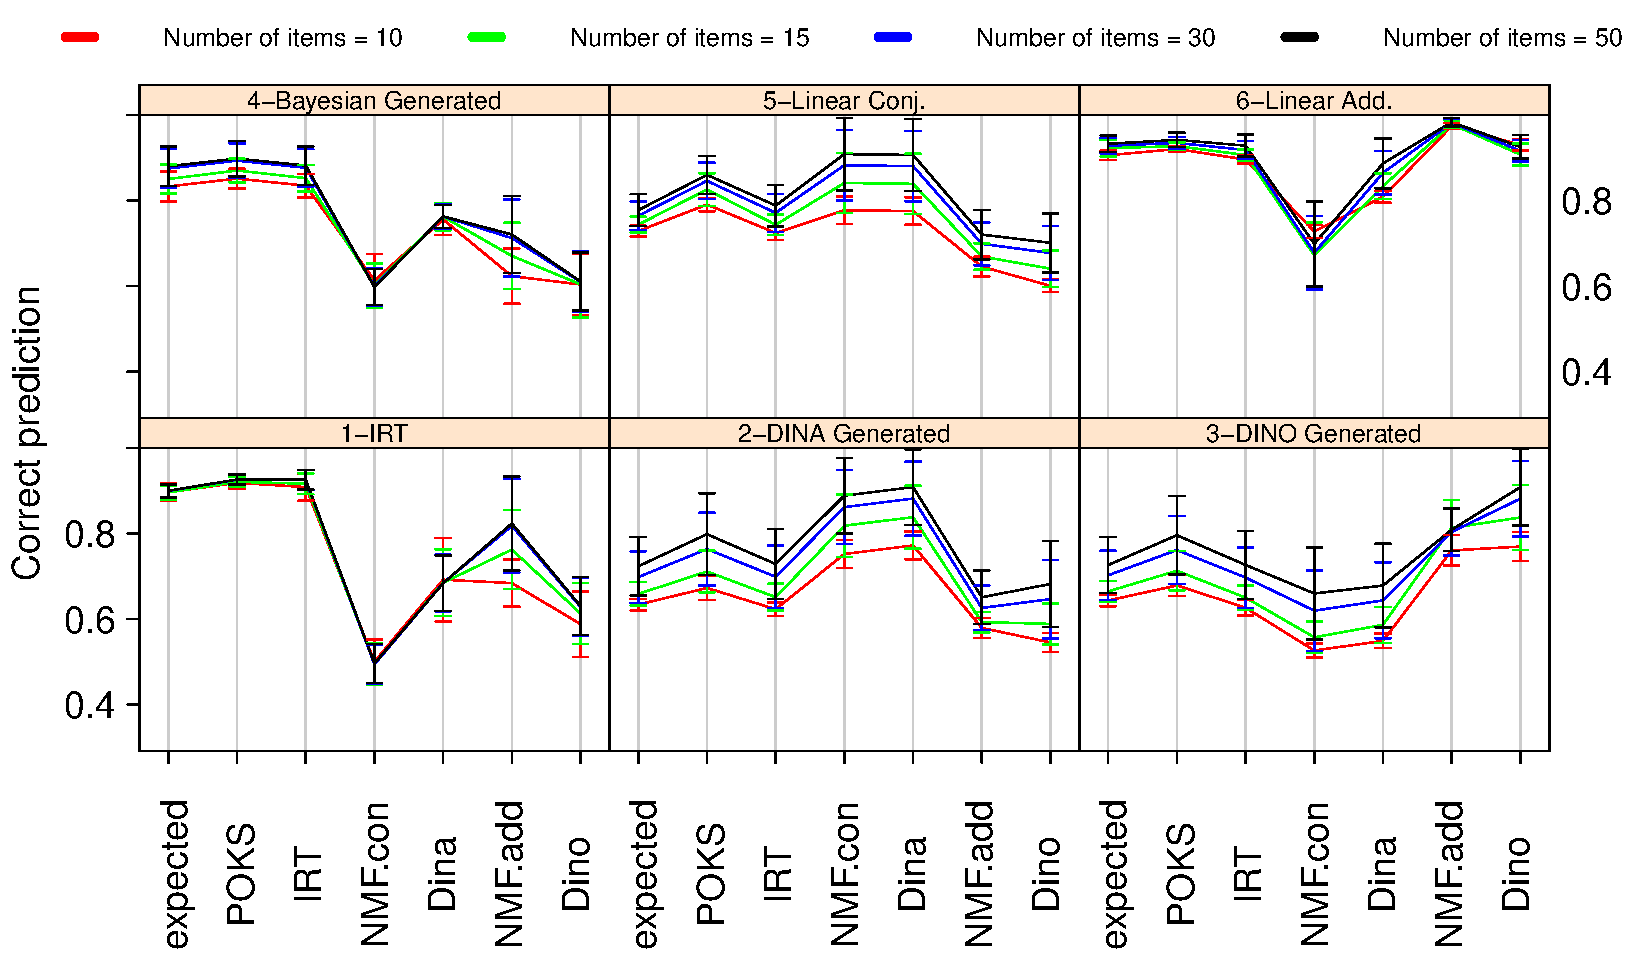
\includegraphics[scale=0.58]{numberofitems.pdf}
\caption{Variation of \textbf{Number of items} Over synthetic data sets}
\label{figNumberofItems}
\end{figure}

\begin{figure}
  \centering
    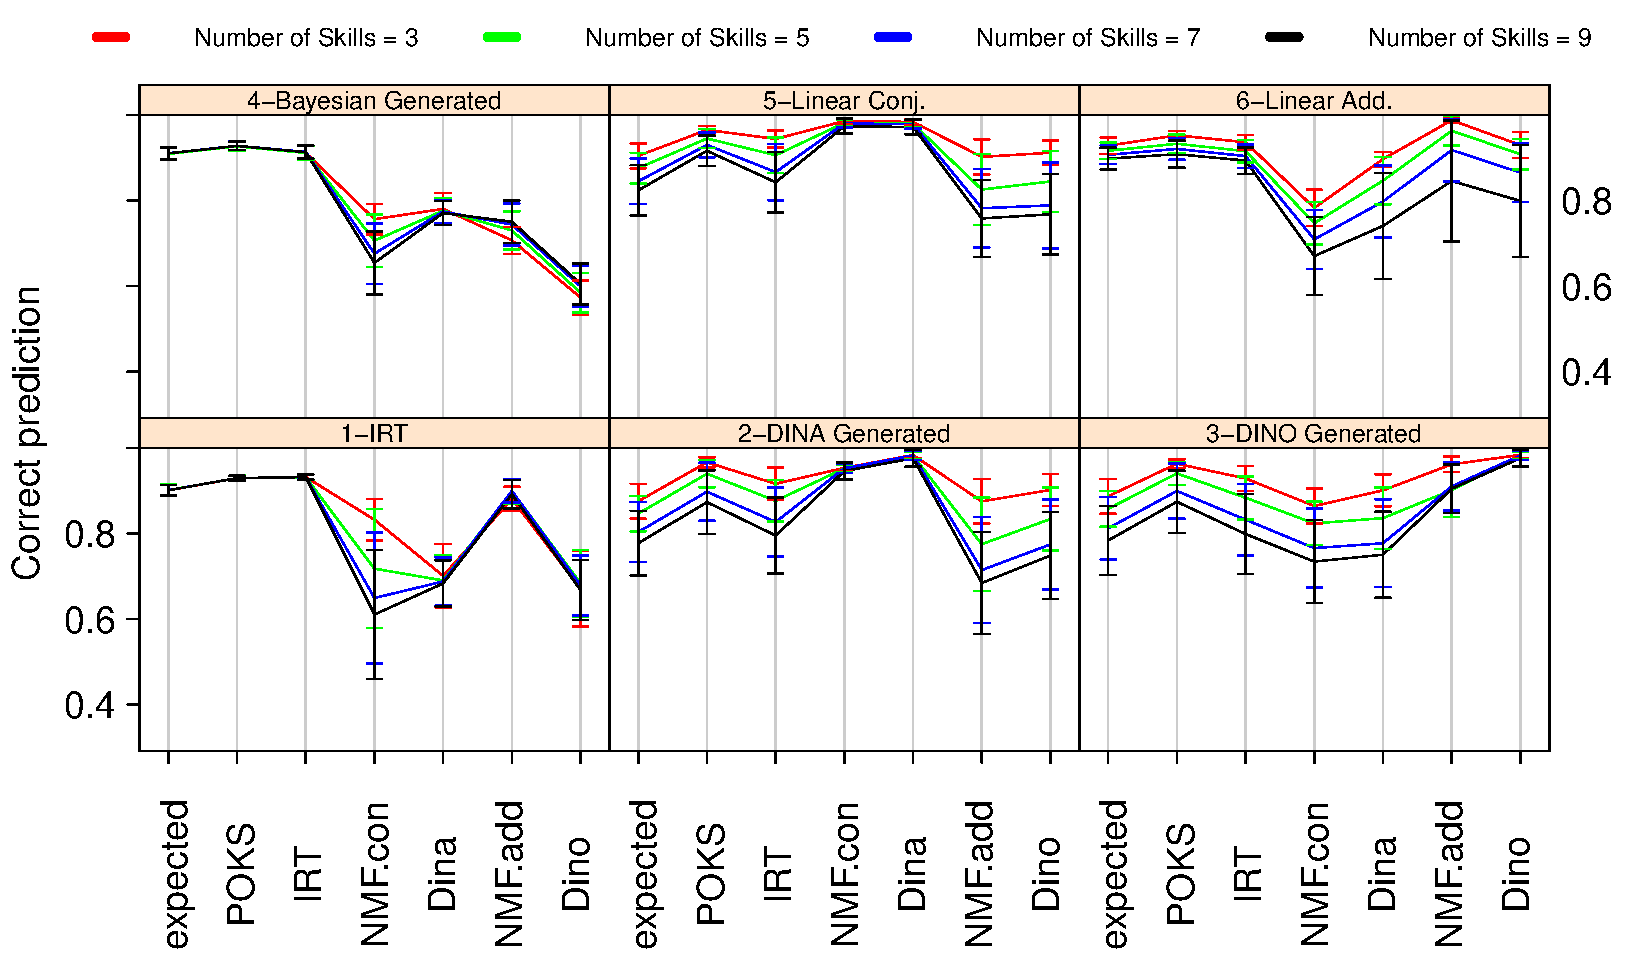
\includegraphics[scale=0.58]{numberofskills.pdf}
\caption{Variation of \textbf{Number of skills} Over synthetic data sets}
\label{figSkills}
\end{figure}

\begin{figure}
  \centering
    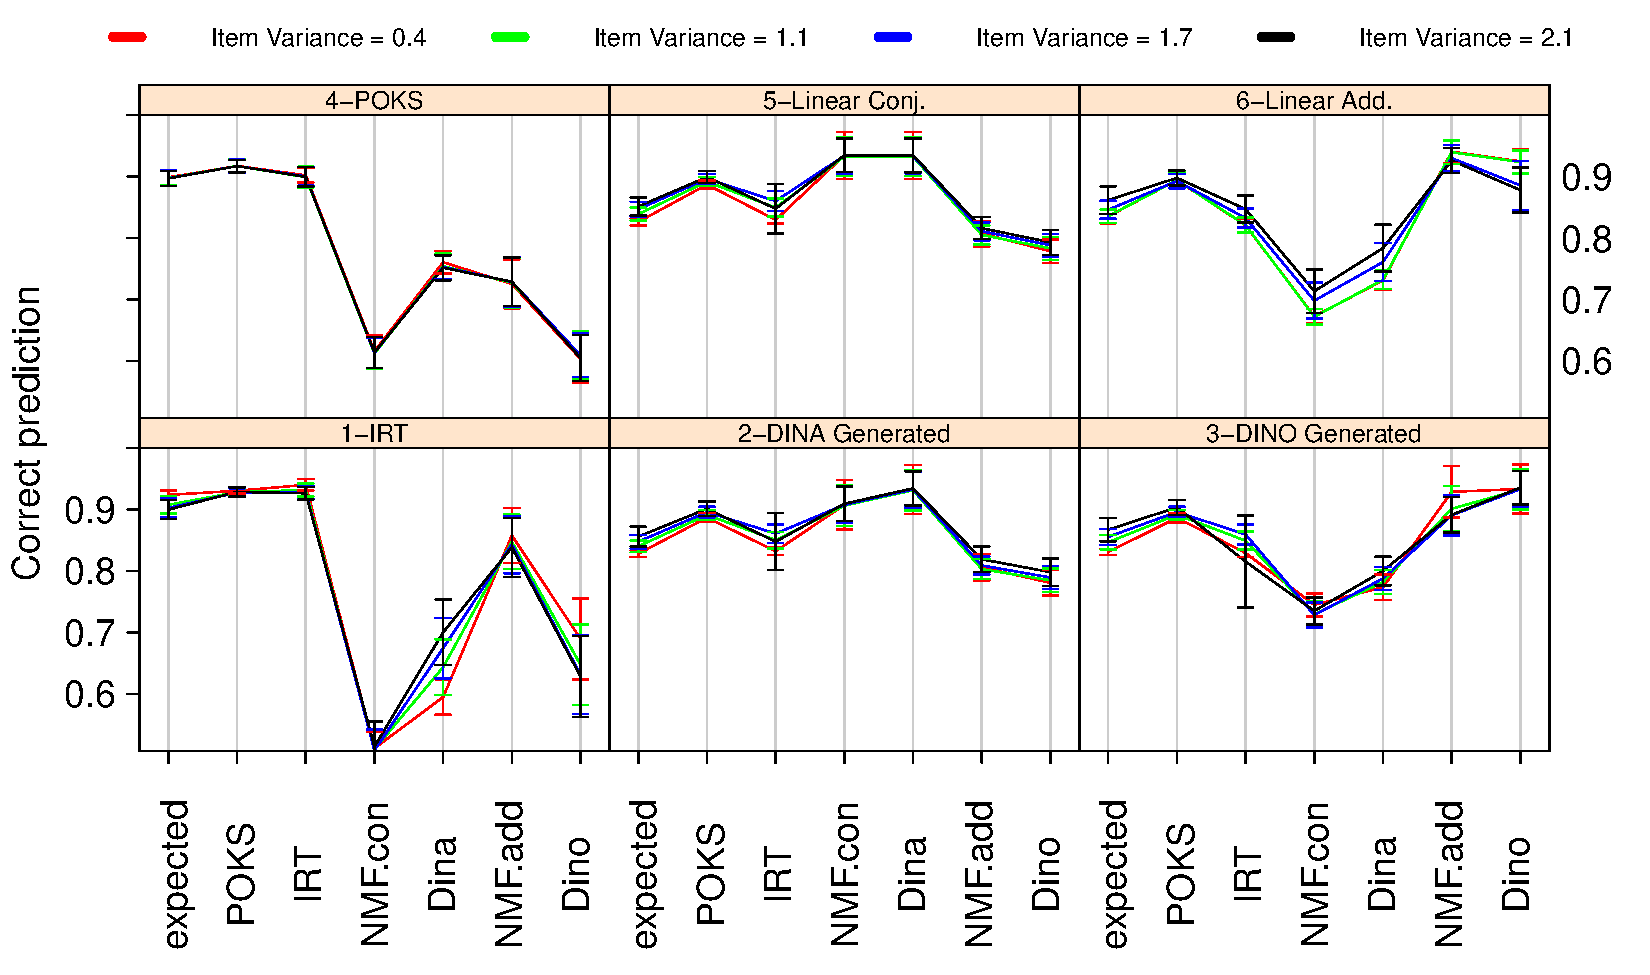
\includegraphics[scale=0.58]{ItemVariance.pdf}
\caption{Variation of \textbf{Item Variance} Over synthetic data sets}
\label{figitemVar}
\end{figure}

\begin{figure}
  \centering
    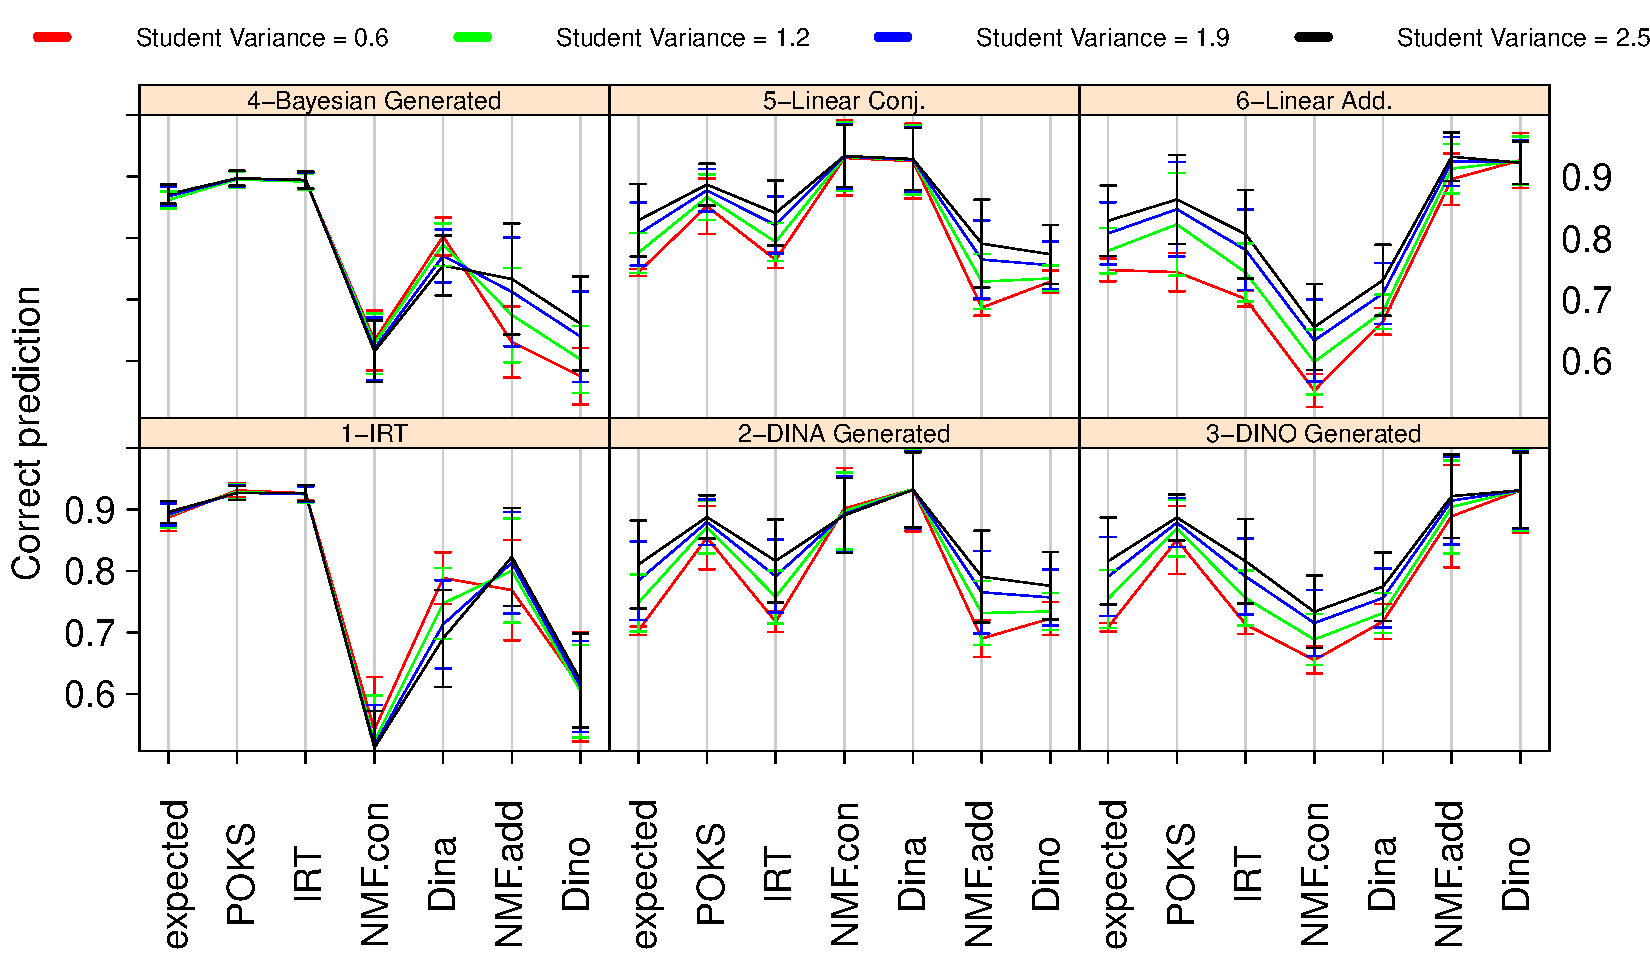
\includegraphics[scale=0.58]{StudentVariance.pdf}
\caption{Variation of \textbf{Student variance} Over synthetic data sets}
\label{figStudentVar}
\end{figure}


\begin{figure}
  \centering
    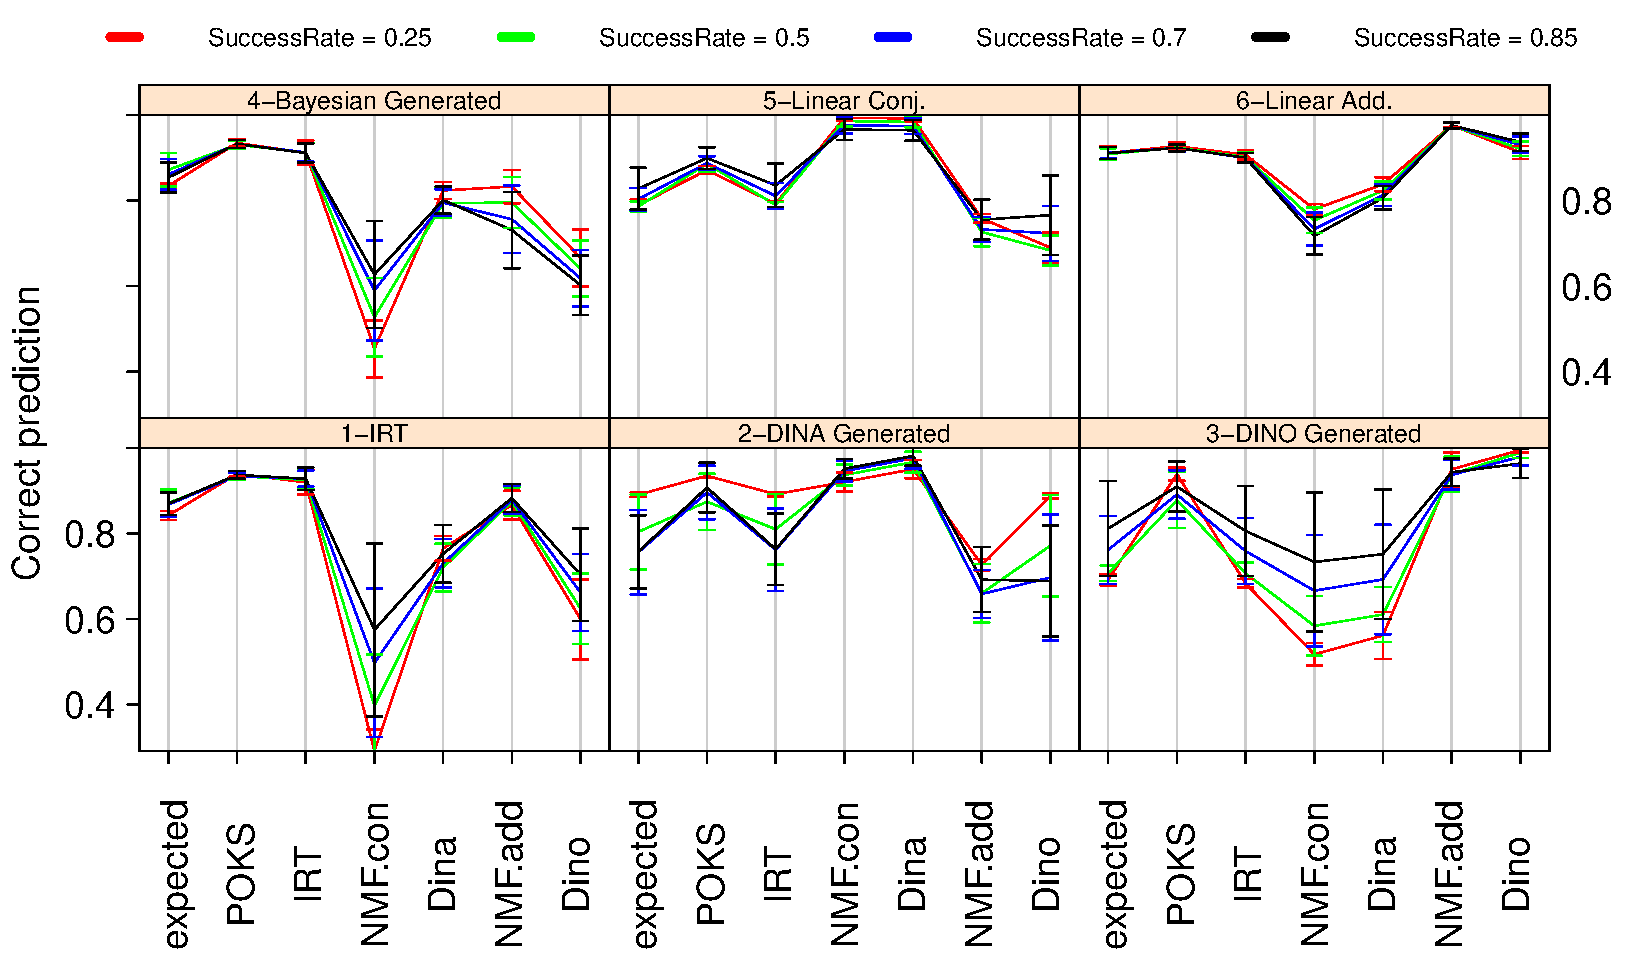
\includegraphics[scale=0.58]{Successrate.pdf}
\caption{Variation of \textbf{Success Rate} Over synthetic data sets}
\label{figSucceessRate}
\end{figure}

\note{Here again, some details are missing.  What are the Q-matrices?  How are the matrices with different number of skills obtained?  Maybe in the discussion later, or here, questions such as ``what if we have matrices with different number of items per skills, in particular one skill per item?}

The next parameter is the number of skills which is a latent parameter. Figure~\ref{figSkills} shows the results of running experiment 1 on datasets with different number of latent skills. Synthetic data based on IRT and POKS can not be affected by this parameter because they are either zero or one skill models. However in the learning phase of these datasets this parameter is required. The signature pattern did not change substantially for these datasets except for linear conjunctive model. For other datasets the signature pattern stays stable while it slightly shifts upward on the correct prediction axis as the number of skills degrades. Increasing the number of skills while the number of item is constant can resemble the single skill modeling such as IRT and POKS. 

%%%%Need to be restat from :%%%%%

Figure~\ref{figitemVar} shows the same experiment across datasets with different item variance. The item variance was reflected as the item difficulty for IRT and initial odds for POKS. Clearly the pattern stays the same for different values except for few minor changes. Although the the set of performance values shifts across the correct prediction axis but the pattern stays the same.

Finally, we did a last experiment on datasets with different success rates. For synthetic data, the success rate starts from 0.25\% up to 0.85\%. The pattern is scaled for some linear methods on IRT and bayesian generated data and it doesn't change the performance of IRT and POKS themselves. For datasets with multi-skills model's ground truth the signature was shifted downward on these models predictive performance as the success rate of synthetic data degrades.



%Still we can see that the highest performance is the same model behind the generated dataset. 

%%%%Need to be restat to :%%%%

\section{Results of Experiment 3: Model selection based on performance vector classification}
 
\note{``Prototype'' is used but not explained...}

The third experiment addresses the question of identifying the ground thruth model using performance signatures.
As explained before, the uniqueness characteristic of synthetic data signatures offers a means to identify the ground truth based on the similarity between the prototype performance from a synthetic data and the target performance vector from the real data. In this experiment we used the measure form section \ref{Sigapproach-measure} as a degree of similarity between these vectors.

\note{I started rephrasing but I do not understand very well so the rephrasing may not be correct...}

In this experiment, a number of synthetic data sets for each model are created using different parameters. There are $6$ data specific parameters (namely : Number of items, students, skills, average success rate, item and student score variance) and $4$ different values for each parameter.  In total, this makes $24$ combinations of unique parameter-value pairs.  We will call a combination a \textbf{group}. For each each group, we generate $10$ datasets with different seeding point for each skills assessment ground truths. In total, $24$ samples are generated.  

\note{Next paragrapy not clear...  What is correlated with what?  How about using mathematical notation for making this clearer?  Also defining how a ``prototype'' is defined.}

According to the condition of the signature model selection approach we are permitted to calculate the correlation table among the members of each group. The expectation is that those vectors with same model show high correlation. Table~\ref{tablSyn} shows the average correlation table of these $24$ groups.

\subsection{Results}

\note{Here too I tried to rephrase but I am not sure I have the right version and some details are missing.  Please use a mathematical notation to make things clearer on how prototypes are calculated, how correlations are obtained, etc. }

We evaluate the value of the correlation between performance vectors as an indicator of model fit. The diagonal of table~\ref{tablSyn} shows the correlation between the performance vectors of the model that was used to create the synthetic data. As expected, it shows high correlations because it compares the same model generated datasets. On the other hand some models such as IRT and POKS also show a high correlation since they are not using multi-skills models. Those models that share concepts such as DINA and NMF conjunctive also show a high correlation comparing to other models because they are linear models which deal with conjunctive model of Q-matrix. DINO and NMF additive has almost a high correlation but since the additive model is slightly different from the disjunctive model then they are less correlated.

In general, correlation similarity provides a very good measure of model fit, although models that have strong similarities show close values that could lead to misrecognition among them, which is to be expected.

\begin{table}[h]
\center
\begin{tabular}{c|c|c|c|c|c|c|c|}
\multicolumn{2}{c}{} & \multicolumn{6}{c}{Synthetic Datasets} \tabularnewline
\multicolumn{8}{c}{} \tabularnewline
\cline{3-8} 
\multicolumn{2}{c|}{} & POKS & IRT & NMF Conj. & DINA & NMF Add. & DINO\tabularnewline
\cline{2-8}
\cline{2-3}
&POKS & \textbf {0.96} & \multicolumn{1}{|c}{} & \multicolumn{1}{c}{} & \multicolumn{1}{c}{} & \multicolumn{1}{c}{}\tabularnewline
\cline{2-4}
&IRT & 0.86 & \textbf {0.96} & \multicolumn{1}{|c}{} & \multicolumn{1}{c}{} & \multicolumn{1}{c}{} & \multicolumn{1}{c}{}\tabularnewline
\cline{2-5}
&NMF Conj. & 0.22 & -0.20 & \textbf {0.96} & \multicolumn{1}{|c}{} & \multicolumn{1}{c}{} & \multicolumn{1}{c}{}\tabularnewline
\cline{2-6}
&DINA & 0.02 & -0.40 & 0.94 & \textbf {0.96} & \multicolumn{1}{|c}{} & \multicolumn{1}{c}{}\tabularnewline
\cline{2-7}
&NMF Add. & 0.44 & 0.75 & -0.62 & -0.73 & \textbf {0.93} & \multicolumn{1}{|c}{}\tabularnewline
\cline{2-8}
\multicolumn{1}{c|}{\multirow{-6}{*}{\begin{sideways}Synthetic Datasets\end{sideways}}}&DINO & -0.15 & 0.20 & -0.70 & -0.69 & 0.63 & \textbf {0.95}\tabularnewline
\cline{2-8}
\end{tabular}
\caption{Degree of similarity between six synthetic datasets based on the correlation}
\label{tablSyn}
\end{table}

\begin{table}[h]
 \center
\begin{tabular}{c|c|c|c|c|c|c|c|c|}

\multicolumn{2}{c}{}&\multicolumn{7}{c}{Real Datasets}\tabularnewline   
\multicolumn{9}{c}{}\tabularnewline   
\cline{6-9}
\multicolumn{5}{c|}{}&\multicolumn{4}{c|}{Fraction subsets}   \tabularnewline   
\cline{3-9} 
\multicolumn{2}{c|}{}   & Vomlel &ECPE &Fraction &1&21&22&23\tabularnewline
\cline{2-9}
\cline{2-9}
&Random & 0.58 &\textbf {0.73} & 0.61   & 0.43 & 0.24 & 0.61 & 0.57 \tabularnewline
\cline{2-9}
&IRT & \textbf {0.90} & 0.42 & 0.72   & 0.88 & 0.60 & 0.77 & 0.61 \tabularnewline
\cline{2-9}
&DINA & -0.38  & -0.09 &   0.23 &   0.30 & 0.56 & 0.06 & 0.38 \tabularnewline
\cline{2-9}
&DINO & 0.34 & 0.15  &  -0.18 &  -0.31 & 0.10 & -0.08 & 0.38 \tabularnewline
\cline{2-9}
&POKS & 0.75 &0.40  &  \textbf {0.83}  &  \textbf {0.95} &\textbf {0.70} & \textbf {0.83} & \textbf {0.80}\tabularnewline
\cline{2-9}
 &NMF Conj. & -0.05 & 0.54  & 0.51   & 0.55  & 0.66 & 0.33 & 0.57\tabularnewline
\cline{2-9}
\multicolumn{1}{c|}{\multirow{-7}{*}{\begin{sideways}Synthetic Datasets\end{sideways}}}&NMF Add. & 0.39 &0.06   & -0.04   & -0.19 & -0.03 & 0.13 & 0.28\tabularnewline
\cline{2-9}
\end{tabular}
\caption{Degree of similarity between six synthetic datasets and the ground truth based on the correlation}
\label{tablSynReal}
\end{table}

Table~\ref{tablSynReal} shows the correlation of target performance vector of the real data in columns with prototype performance vector of synthetic data generated with underlying model in rows. Vomlel dataset shows a high correlation with IRT model and Fraction with its subset datasets show similarity with POKS model. As expected ECPE has the highest correlation with random generated dataset.

%%%%%%%%%%%%%%%%%%%%%%%%%%%%%%%%%%%%%%%%%%%%%%%%%%%%%%%%%%%%%%%%%%%%%%%%%%%%%

\section{Results of Experiment 4: Generality of the signature approach under different assumptions about the data}
\label{GeneralityRes}

Having shown that the correlation similarity between performance vectors is a good indicator of model fit for synthetic data (see Table~\ref{tablSyn}), we now move to the final experiment to evaluate the ability of the approach to identify the ground thruth model and compare the results with the simple best performer approach.

Table~\ref{Classification-Conf} shows the confusion matrix of this experiment. In total, there exists 1440~datasets where each model corresponds to 240 dataset. The gray cells in table~\ref{Classification-Conf} show the true positive values and other values in each column represent the false positive predictions for a group of datasets.The values in each row shows the number of false negative predictions for each model. The confusion is mostly between those techniques that shares same concepts specially between NMF Conjunctive and DINA model where we use conjunctive Q-matrices. 

\begin{table}
\center
\begin{footnotesize}

\begin{adjustwidth}{-0.5cm}{}
\begin{tabular}{c|c!{\VRule[2pt]}c!{\VRule}c!{\VRule[2pt]}c|c!{\VRule[2pt]}c|c!{\VRule[2pt]}c|c!{\VRule[2pt]}c|c!{\VRule[2pt]}c|c!{\VRule[2pt]}c|c|}
\multicolumn{3}{c}{ BP: Best Performer}&\multicolumn{11}{c}{Datasets}&\multicolumn{2}{c}{}\tabularnewline
\cline{15-16}
\multicolumn{3}{c}{ NN: Nearest Neighbor}&\multicolumn{11}{c!{\VRule[2pt]}}{}& \multicolumn{2}{|c|}{Accuracy} \tabularnewline
\cline{3-14}
\multicolumn{2}{c|}{}&\multicolumn{2}{c|}{ POKS}&\multicolumn{2}{c|}{ IRT}&\multicolumn{2}{c|}{ NMF Conj.}&\multicolumn{2}{c|}{ DINA}&\multicolumn{2}{c|}{ NMF Add}&\multicolumn{2}{c!{\VRule[2pt]}}{ DINO}&\multicolumn{2}{c|}{  \scriptsize (\%)}\tabularnewline
\cline{3-16}
\multicolumn{1}{c}{}&\multicolumn{1}{c|}{}&\multicolumn{1}{c|}{ BP}&\multicolumn{1}{c|}{ NN}&\multicolumn{1}{c|}{ BP}&\multicolumn{1}{c|}{ NN}&\multicolumn{1}{c|}{ BP}&\multicolumn{1}{c|}{ NN}&\multicolumn{1}{c|}{ BP}&\multicolumn{1}{c|}{ NN}&\multicolumn{1}{c|}{ BP}&\multicolumn{1}{c|}{ NN}&\multicolumn{1}{c|}{ BP}&\multicolumn{1}{c!{\VRule[2pt]}}{ NN}&\multicolumn{1}{c|}{ BP}&\multicolumn{1}{c|}{ NN}\tabularnewline
\cline{3-16}
\cline{3-16}
\cline{2-16}
\multicolumn{1}{c|}{}& Expected& 0& 0& 0& 0& 0& 0& 0& 0&12& 0& 2& 0& & \tabularnewline
\cline{2-16}
\multicolumn{1}{c|}{}& POKS&\cellcolor{gray!25} 238&\cellcolor{gray!25} 218&130&32&21& 12&14& 0&18&13& 1& 0&85&95\tabularnewline
\cline{2-16}
\multicolumn{1}{c|}{}& IRT& 2& 20&\cellcolor{gray!25}110&\cellcolor{gray!25}208& 0& 0& 0& 0& 0&15& 0& 3&100&97\tabularnewline
\cline{2-16}
\multicolumn{1}{c|}{}& NMF \scriptsize Conj.& 0& 0& 0& 0&\cellcolor{gray!25}82&\cellcolor{gray!25}180& 5&73& 0& 0& 0& 0&100&94\tabularnewline
\cline{2-16}
\multicolumn{1}{c|}{}& DINA& 0& 0& 0& 0&137&48&\cellcolor{gray!25}221&\cellcolor{gray!25}167& 0& 0& 0& 0&87&96\tabularnewline
\cline{2-16}
\multicolumn{1}{c|}{}& NMF \scriptsize Add.& 0& 2& 0& 0& 0& 0& 0& 0&\cellcolor{gray!25}210&\cellcolor{gray!25}211& 14&10&99&99\tabularnewline
\cline{2-16}
\multicolumn{1}{c|}{\multirow{-7}{*}{\begin{sideways}Models\end{sideways}}}& DINO& 0& 0& 0& 0& 0& 0& 0& 0& 0& 1&\cellcolor{gray!25}223&\cellcolor{gray!25}227&100&100\tabularnewline
\cline{1-16}
\multicolumn{2}{|c!{\VRule[2pt]}}{ Accuracy \scriptsize (\%)} & 99 & 91 & 46 & 87 &34 & 75 & 92 & 70 & 88 & 87 & 93 & 95&\multicolumn{2}{|c}{}\tabularnewline
\cline{1-14}
\end{tabular}
\end{adjustwidth}

\end{footnotesize}

\caption{Confusion matrix for classification of 210 synthetic datasets on 7 models with Best performer Vs. Nearest neighbor methods}
\label{Classification-Conf}
\end{table}

The accuracy that is reported in the last row of table~\ref{Classification-Conf} is calculated based on $\frac{TP}{240}$ which counts the true positive predictions for each sub set of datasets with the same actual ground truth. The accuracy that is reported in the last two columns of table~\ref{Classification-Conf} shows how faithful the classification method is in the sense of specificity. Therefore it counts true negative values based on $\frac{TN}{1200}$ (1200 is the number of datasets that have ground truth oppose to the target model). In terms of true positive selections there is no benefit between any of these methods even sometimes best performer shows to perform better (specially for DINA and IRT).

\note{Why does the last row of table\ref{Classification-Acc} has 4 grey cells?}

Taking into account the false negative and false positive values changes the classification results. Table~\ref{Classification-Acc} shows the accuracy of this classification in terms of precision, recall, $F1$ measure and accuracy ($\frac{TN+TP}{1440}$). Since $F1$ measure is combining both precision and recall, then it is a good measure to show the comparison. The third column of each classification method shows that F-measure is increased when the signature approach is used for classification which is almost close to $1$. Also in terms of individual scores per method we also report accuracy of each technique which considers true positive and true negative values. The last column of table~\ref{Classification-Acc} shows this result. The total accuracy which considers true positive numbers over number of datasets regardless of individual models shows that the best performer approach gets $0.75\%$ and the signature approach gets upto $0.84\%$ of accuracy.


\begin{table}[h]
\center	
%\begin{scriptsize}
\begin{tabular}{c|c|c|c|c|c!{\VRule[2pt]}c|c|c|c|}
\multicolumn{2}{c}{}&\multicolumn{8}{c}{Performance}\tabularnewline
\cline{3-10}
\multicolumn{2}{c|}{}&\multicolumn{4}{c|}{Best Performer}&\multicolumn{4}{c|}{Nearest Neighbor}\tabularnewline
\cline{3-10}
\multicolumn{2}{c|}{}&\scriptsize Precision&\scriptsize Recall&\multicolumn{1}{c|}{\scriptsize F-Measure}&\scriptsize Accuracy&\scriptsize Precision&\scriptsize Recall&\scriptsize F-Measure&\scriptsize Accuracy\tabularnewline
\cline{2-10}
&POKS&0.564&0.992&0.719&0.871&0.793&0.908&\cellcolor{gray!25}0.847&\cellcolor{gray!25}0.945\tabularnewline
\cline{2-10}
&IRT&0.982&0.458&0.625&0.908&0.846&0.867&\cellcolor{gray!25}0.856&\cellcolor{gray!25}0.951\tabularnewline
\cline{2-10}
&NMF Conj.&0.943&0.342&0.502&0.887&0.711&0.750&\cellcolor{gray!25}0.730&\cellcolor{gray!25}0.907\tabularnewline
\cline{2-10}
&DINA&0.617&0.921&0.739&0.891&0.777&0.696&\cellcolor{gray!25}0.734&\cellcolor{gray!25}0.916\tabularnewline
\cline{2-10}
&NMF Add.&0.938&0.875&0.905&0.969&0.946&0.879&\cellcolor{gray!25}0.911&\cellcolor{gray!25}0.971\tabularnewline
\cline{2-10}
\multicolumn{1}{c|}{\multirow{-7}{*}{\begin{sideways}Models\end{sideways}}}&DINO&1&0.929&\cellcolor{gray!25}0.963&\cellcolor{gray!25}0.988&0.996&0.946&\cellcolor{gray!25}0.970&\cellcolor{gray!25}0.990\tabularnewline
\cline{2-10}
\end{tabular}
\caption{Accuracy of best performer and nearest neighbor classification methods  }
\label{Classification-Acc}
\end{table}
